\documentclass[10pt, aspectratio=43]{beamer}

% --- Pacotes Básicos ---
\usepackage[utf8]{inputenc}
\usepackage[T1]{fontenc}
\usepackage[brazilian]{babel}
\usepackage{amsmath, amssymb, amsthm}
\usepackage{listings}
\usepackage{xcolor}
\usepackage{tikz}
\usepackage{tcolorbox}
\usepackage{booktabs} % \toprule, \midrule, \bottomrule usados na tabela de resultados
\usepackage[alf]{abntex2cite}
\setbeamertemplate{caption}[numbered]

% --- Configuração Visual IDÊNTICA ao PDF 09-logic-in-lean ---
\usetheme{Singapore} % Tema nativo que gera o degradê e os miniframes exatamente como no PDF
\setbeamertemplate{navigation symbols}{} % Remove ícones de navegação inferiores

% Cores originais do Beamer/PDF
\definecolor{pucblue}{RGB}{51, 51, 179} % Azul clássico do Beamer (structure) usado no PDF
\definecolor{commentgreen}{RGB}{0, 110, 0}
\definecolor{keywordblue}{RGB}{0, 0, 180}

\setbeamercolor{structure}{fg=pucblue}
\setbeamercolor{title}{fg=pucblue}
\setbeamercolor{frametitle}{fg=pucblue}
\setbeamercolor{section in head/foot}{fg=pucblue}

% Ajusta a cor do degradê do tema Singapore para o tom suave do PDF
\colorlet{beamer@blendedblue}{pucblue}

% Estilo reutilizável para as caixas (tcolorbox); evita repetir as cores em cada slide
\tcbset{
  pucbox/.style={colback=pucblue!5!white, colframe=blue!75!black}
}

% --- Bolinhas vazadas no cabeçalho e marcadores redondos ---
\setbeamertemplate{mini frames}[circle]
\setbeamertemplate{itemize items}[circle]
\setbeamertemplate{enumerate items}[default]
\setbeamertemplate{sections/subsections in toc}[sections numbered]

% Título dos slides alinhado à esquerda (o tema Singapore centraliza por padrão)
\setbeamertemplate{frametitle}[default][left]

% Rodapé limpo apenas com numeração X/Y em negrito na direita (oculto quando sem número)
\setbeamertemplate{footline}{%
  \hfill \textbf{\insertframenumber/\inserttotalframenumber} \hspace{0.3cm} \vspace{0.2cm}
}

% Slide de Sumário automático no início de cada seção (sem contar nem exibir número de página, igual ao PDF)
\AtBeginSection[]{
  {
    \setbeamertemplate{footline}{}
    \begin{frame}[noframenumbering]{Sumário}
      \tableofcontents[currentsection]
    \end{frame}
  }
}

% --- Configuração de Caixas de Código para Lean 4 (Fundo branco e borda fina, igual ao PDF) ---
\lstdefinelanguage{Lean4}{
  keywords={def, theorem, lemma, example, structure, inductive, where, by, intro, apply, exact, rw, cases, with, assumption, rfl, sorry, exfalso, contradiction, forall, exists, Prop, Type, Nat, Bool, List, False, True, And, Or, Not, Injective},
  keywordstyle=\color{keywordblue}\bfseries,
  comment=[l]{--},
  commentstyle=\color{commentgreen}\ttfamily,
  basicstyle=\ttfamily\footnotesize\color{pucblue!90!black},
  backgroundcolor=\color{white},
  frame=single,
  rulecolor=\color{black},
  framesep=4pt,
  xleftmargin=4pt,
  xrightmargin=4pt,
  showstringspaces=false,
  breaklines=true,
  literate=
    {→}{{$\rightarrow$}}1
    {←}{{$\leftarrow$}}1
    {↔}{{$\leftrightarrow$}}1
    {∀}{{$\forall$}}1
    {∃}{{$\exists$}}1
    {∧}{{$\wedge$}}1
    {∨}{{$\vee$}}1
    {¬}{{$\neg$}}1
    {≠}{{$\neq$}}1
    {≤}{{$\le$}}1
    {≥}{{$\ge$}}1
    {α}{{$\alpha$}}1
    {β}{{$\beta$}}1
    {ç}{{\c{c}}}1
    {ã}{{\~a}}1
}

% --- Metadados da Apresentação (Formatação nativa idêntica à capa do PDF) ---
\title[Incompressibilidade e Primos em Lean 4]{Formalização de Limites Inferiores na Distribuição de Primos via Complexidade de Kolmogorov}
\subtitle{\small{Códigos Autodelimitados e o Método da Incompressibilidade em Lean 4}}
\author{Gabriel Resende Machado\texorpdfstring{\\[0.2ex]}{, }{\footnotesize INF2290: Tópicos em Teoria da Computação IV -- Formalização em Lean}}
\institute{\small Departamento de Informática, PUC-Rio}
\date{\tikz[remember picture,overlay] \node[anchor=south, yshift=0.5cm] at (current page.south) {12 de Novembro de 2026};}

\begin{document}

% --- SLIDE DE TÍTULO ---
% Exibe o cabeçalho com degradê, mas omite o número de página no rodapé (como na pág. 1 do PDF)
{
  \setbeamertemplate{footline}{}
  \begin{frame}
    \titlepage
  \end{frame}
}

% --- SUMÁRIO GERAL INICIAL (Igual à pág. 2 do PDF) ---
{
  \setbeamertemplate{footline}{}
  \begin{frame}[noframenumbering]{Sumário}
    \tableofcontents
  \end{frame}
}

% =========================================================================
\section{Introdução}
% =========================================================================

\begin{frame}{O Desafio dos Limites Inferiores}
  Na Teoria da Computação, há uma assimetria fundamental entre dois tipos de problemas:
  \vspace{0.3cm}
  \begin{itemize}
    \item \textbf{Limites Superiores:} para estabelecer um limite superior, basta demonstrar um algoritmo, um circuito ou uma codificação que resolva o problema em espaço ou tempo $T \in O(f(n))$;

    \vspace{2mm}
    \begin{itemize}
        \item O algoritmo \textit{MergeSort} ordena \textit{n} itens com $O(n \log n)$ comparações (afirmação existencial $\exists$).
    \end{itemize}
    
    \vspace{0.2cm}
    \item \textbf{A Dificuldade Assintótica dos Limites Inferiores:} estabelecer um limite inferior $T \in \Omega(f(n))$ exige uma prova universal negativa, \textit{i.e.} demonstrar que \textbf{nenhum} algoritmo possível, sob um determinado modelo computacional, pode ser mais rápido ou compacto que um dado limiar.

    \vspace{2mm}
    \begin{itemize}
        \item Exibir um caminho de 10 km prova que a distância é no máximo 10 km; provar que ela é no mínimo 10 km exige descartar todos os caminhos possíveis (afirmação universal $\forall$).
    \end{itemize}
  \end{itemize}
\end{frame}

\begin{frame}{O Desafio dos Limites Inferiores}
    \begin{figure}
        \centering
        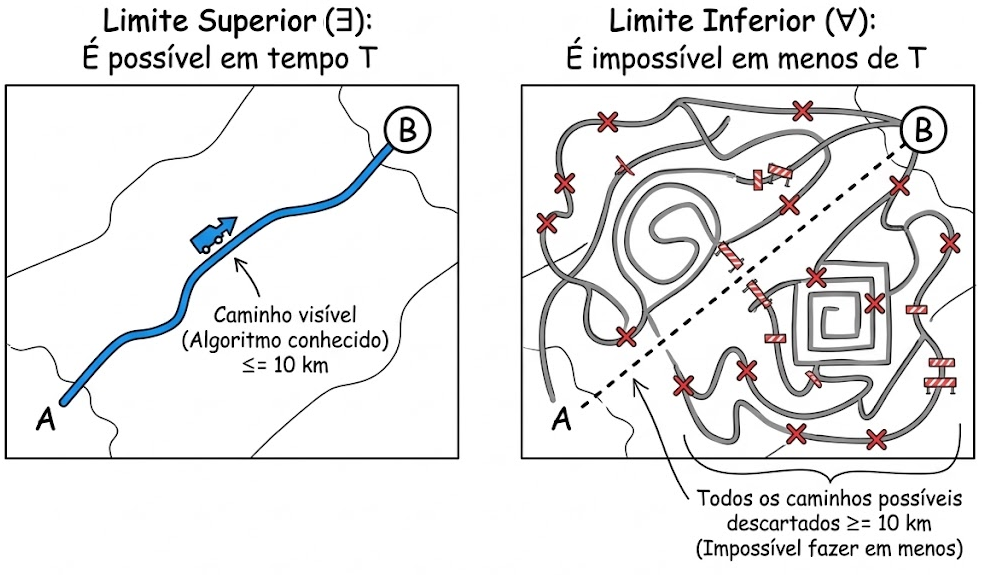
\includegraphics[width=0.95\textwidth]{figures/bounds_example.png}
        \caption{\scriptsize{A assimetria na Teoria da Complexidade. À esquerda, um limite superior prova-se encontrando um único caminho válido. À direita, um limite inferior exige demonstrar que nenhum caminho no universo de possibilidades consegue quebrar a barreira estabelecida.}}
        \label{fig:bounds_example}
    \end{figure}
\end{frame}

\begin{frame}{Regularidade vs. Aleatoriedade}
    \vspace{1mm}
    \begin{itemize}
        \item \small{Um objeto é aleatório se não for possível gerar sua sequência por meio de um programa menor do que ela mesma;}
        \vspace{1mm}
        \item \textbf{\small{Objetos aleatórios são comumente chamados de imcompressíveis via Complexidade de Kolmogorov.}}
    \end{itemize}
    \vspace{1mm}
    \begin{figure}
        \centering
        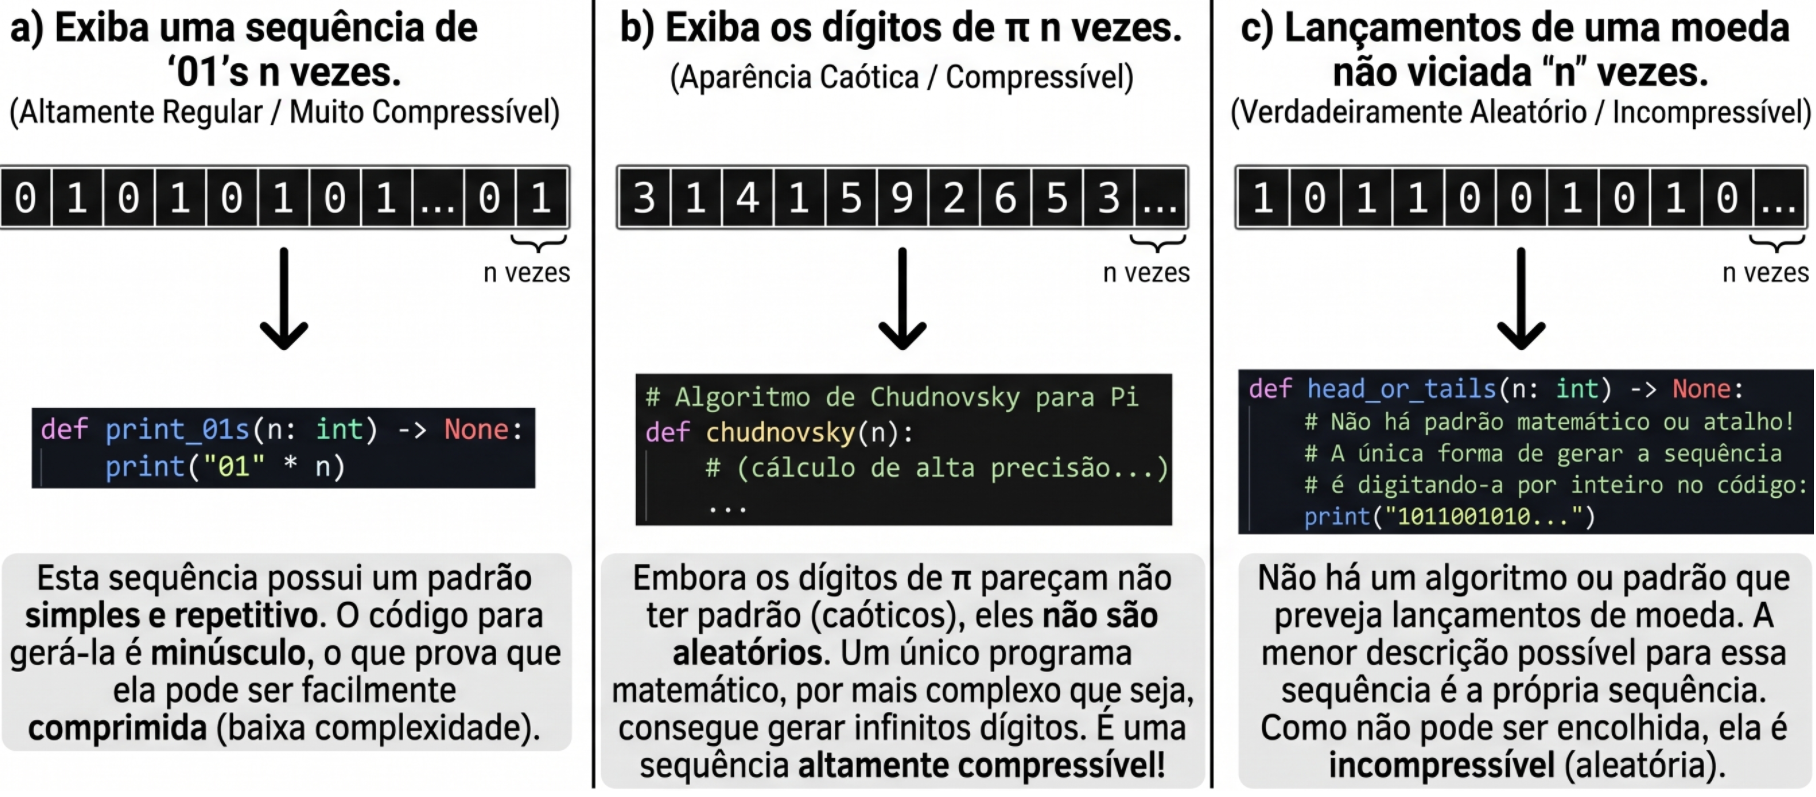
\includegraphics[width=0.98\textwidth]{figures/kolmogorov_examples.png}
        \caption{\footnotesize{Regularidade vs. Aleatoriedade na Complexidade de Kolmogorov: a incompressibilidade algorítmica como a verdadeira medida do que é aleatório.}}
        \label{fig:kolmogorov_examples}
    \end{figure}
\end{frame}

\begin{frame}{A Complexidade de Kolmogorov}
\vspace{2mm}

A Complexidade de Kolmogorov $K(x)$ é o tamanho (em bits) do menor programa que gera $x$, tal que $|x| = n$.

 \begin{tcolorbox}[pucbox, title=Definição Formal]
    \footnotesize{Na Figura \ref{fig:kolmogorov_examples}, nos casos $a)$ e $b)$, as strings de $n$ bits obedeciam a algum padrão ou comportamento reproduzível por meio de um algoritmo de custo adicional $c$ produzir uma saída menor do que $n$. Daí, tem-se:}
    \begin{equation}
        K(x) < n + c
    \end{equation}
    \footnotesize{Contudo, no caso $c)$, não há como reproduzir a saída de $n$ lançamentos de moeda pela sua intrínseca natureza não determinística, a não ser por um algoritmo específico que exiba a própria saída $n$ de lançamentos. Portanto:}
    \begin{equation}
        K(x) \ge n - c
    \end{equation}
    \footnotesize{Como aqui o objetivo é caracterizar sequências que não podem ser significativamente comprimidas, $c$ representa a quantidade máxima de bits que admite-se perder em relação ao comprimento original da sequência.}
 \end{tcolorbox}    
\end{frame}

\begin{frame}{O Princípio da Casa dos Pombos}
\vspace{1mm}
Objetos imcompressíveis -- ou Kolmogorov-Aleatórios -- violam o Princípio da Casa dos Pombos.
    \begin{figure}
        \centering
        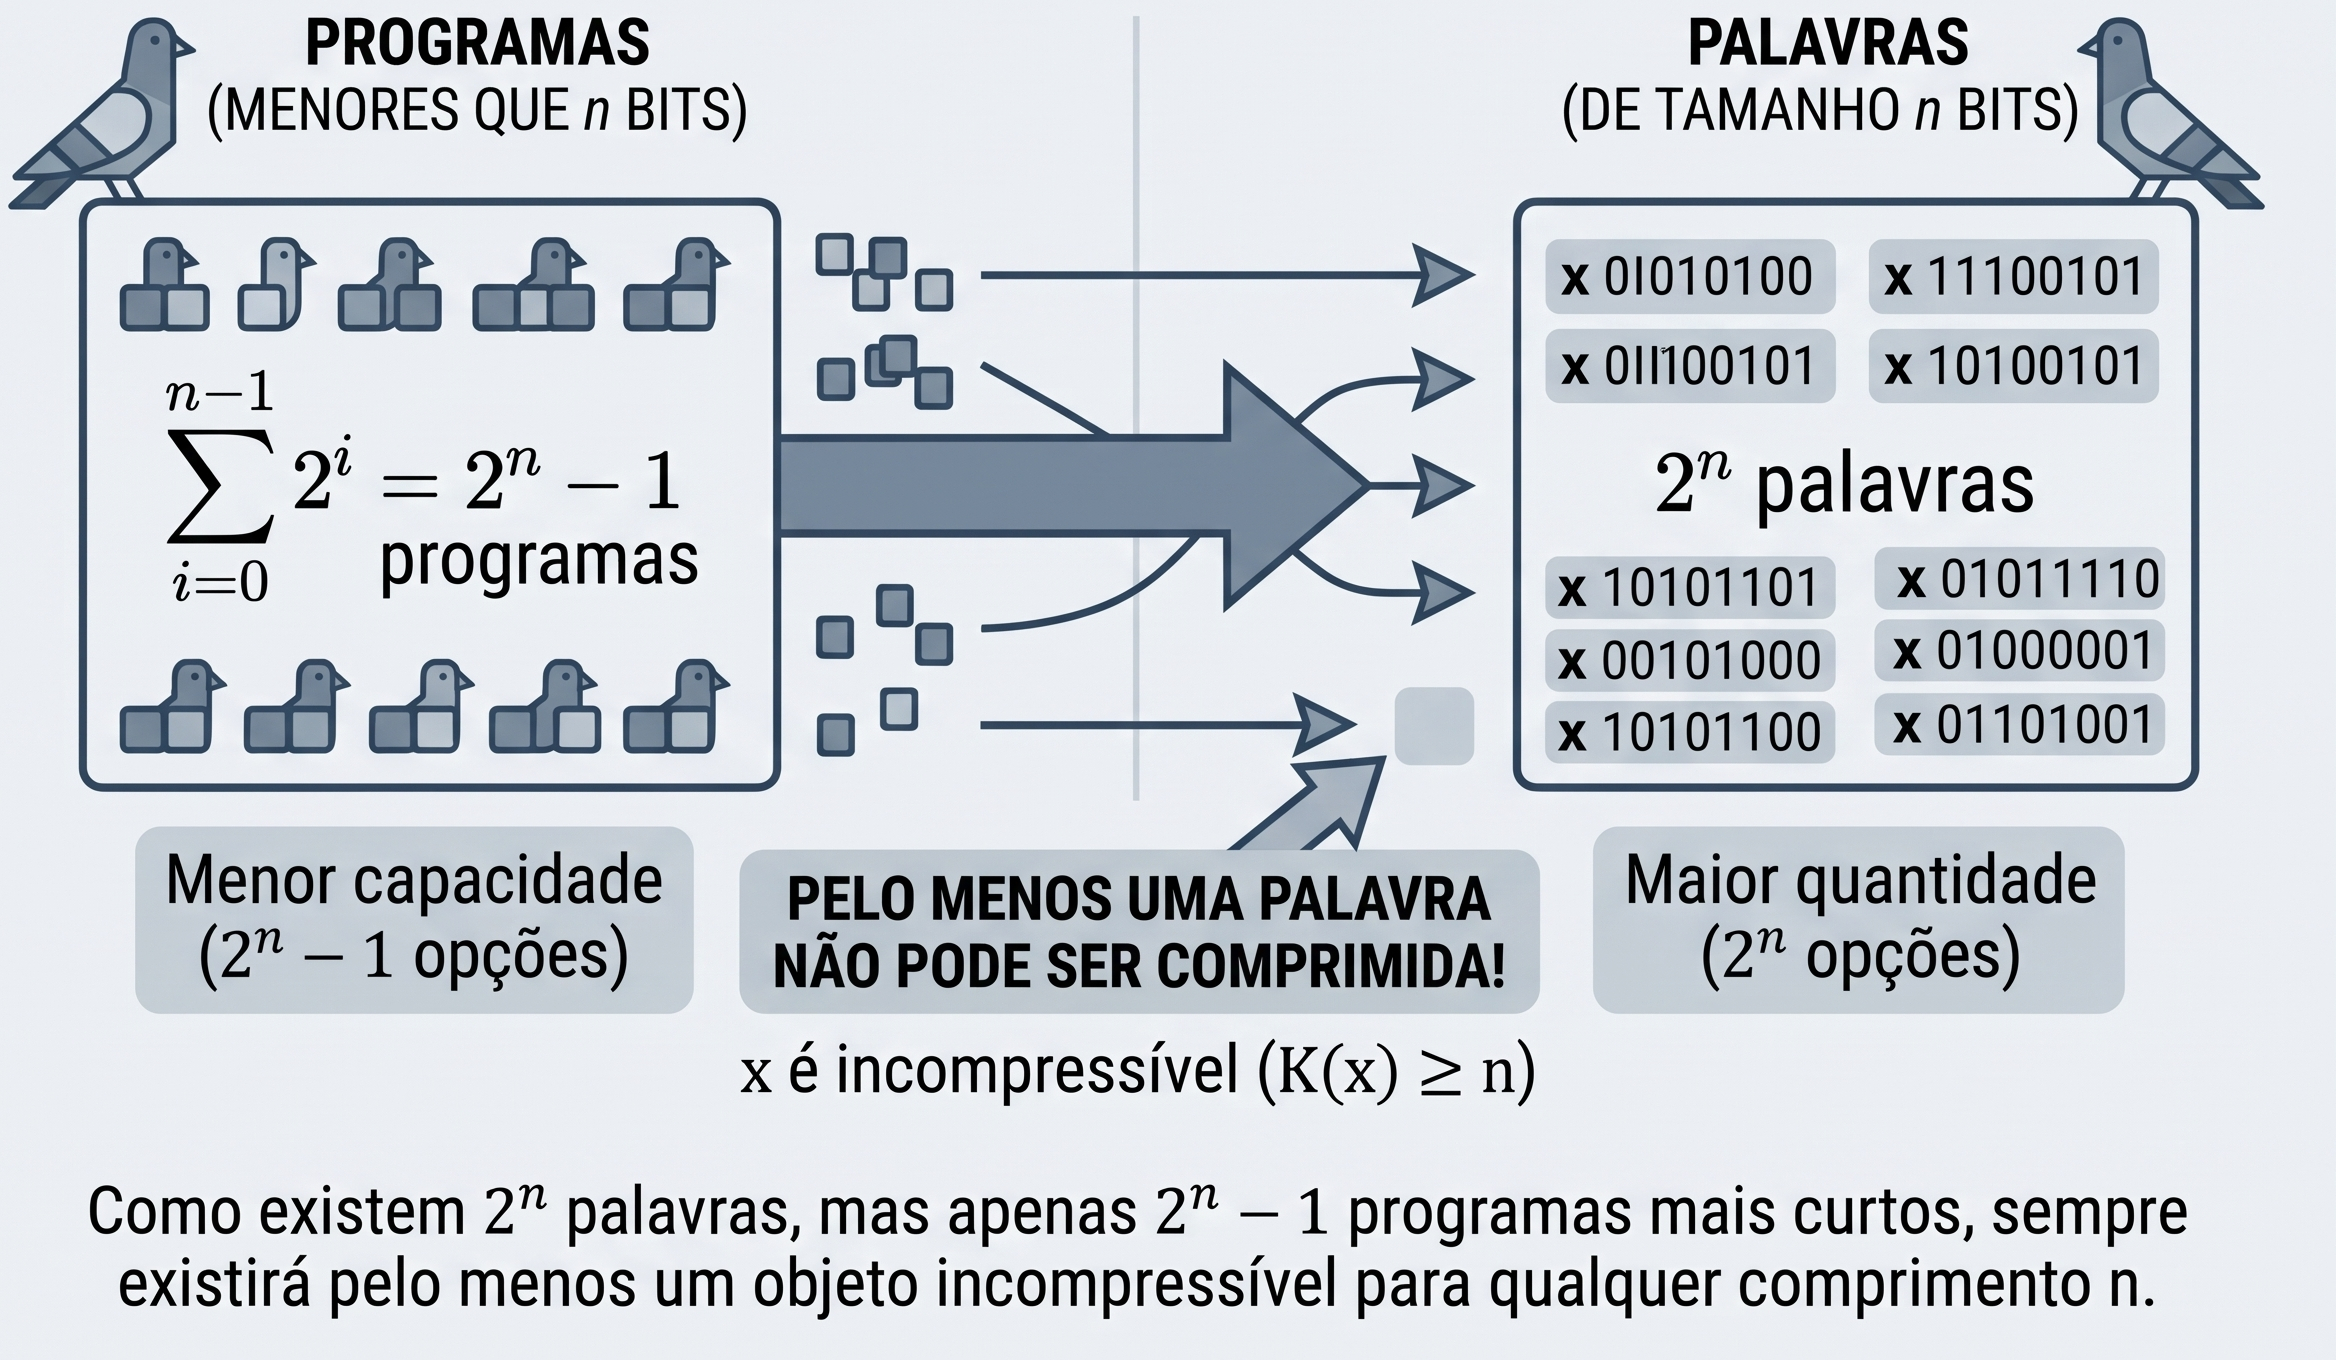
\includegraphics[width=0.95\textwidth]{figures/casa_pombos_definition.jpeg}
        \caption{\footnotesize{A violação do Princípio da Casa dos Pombos em relação à Complexidade de Kolmogorov.}}
        \label{fig:casa_pombos_definition}
    \end{figure}
\end{frame}

\begin{frame}{A Violação do Princípio em Strings $2^n$, sendo $n=4$}
\vspace{1mm}

\begin{figure}
    \centering
    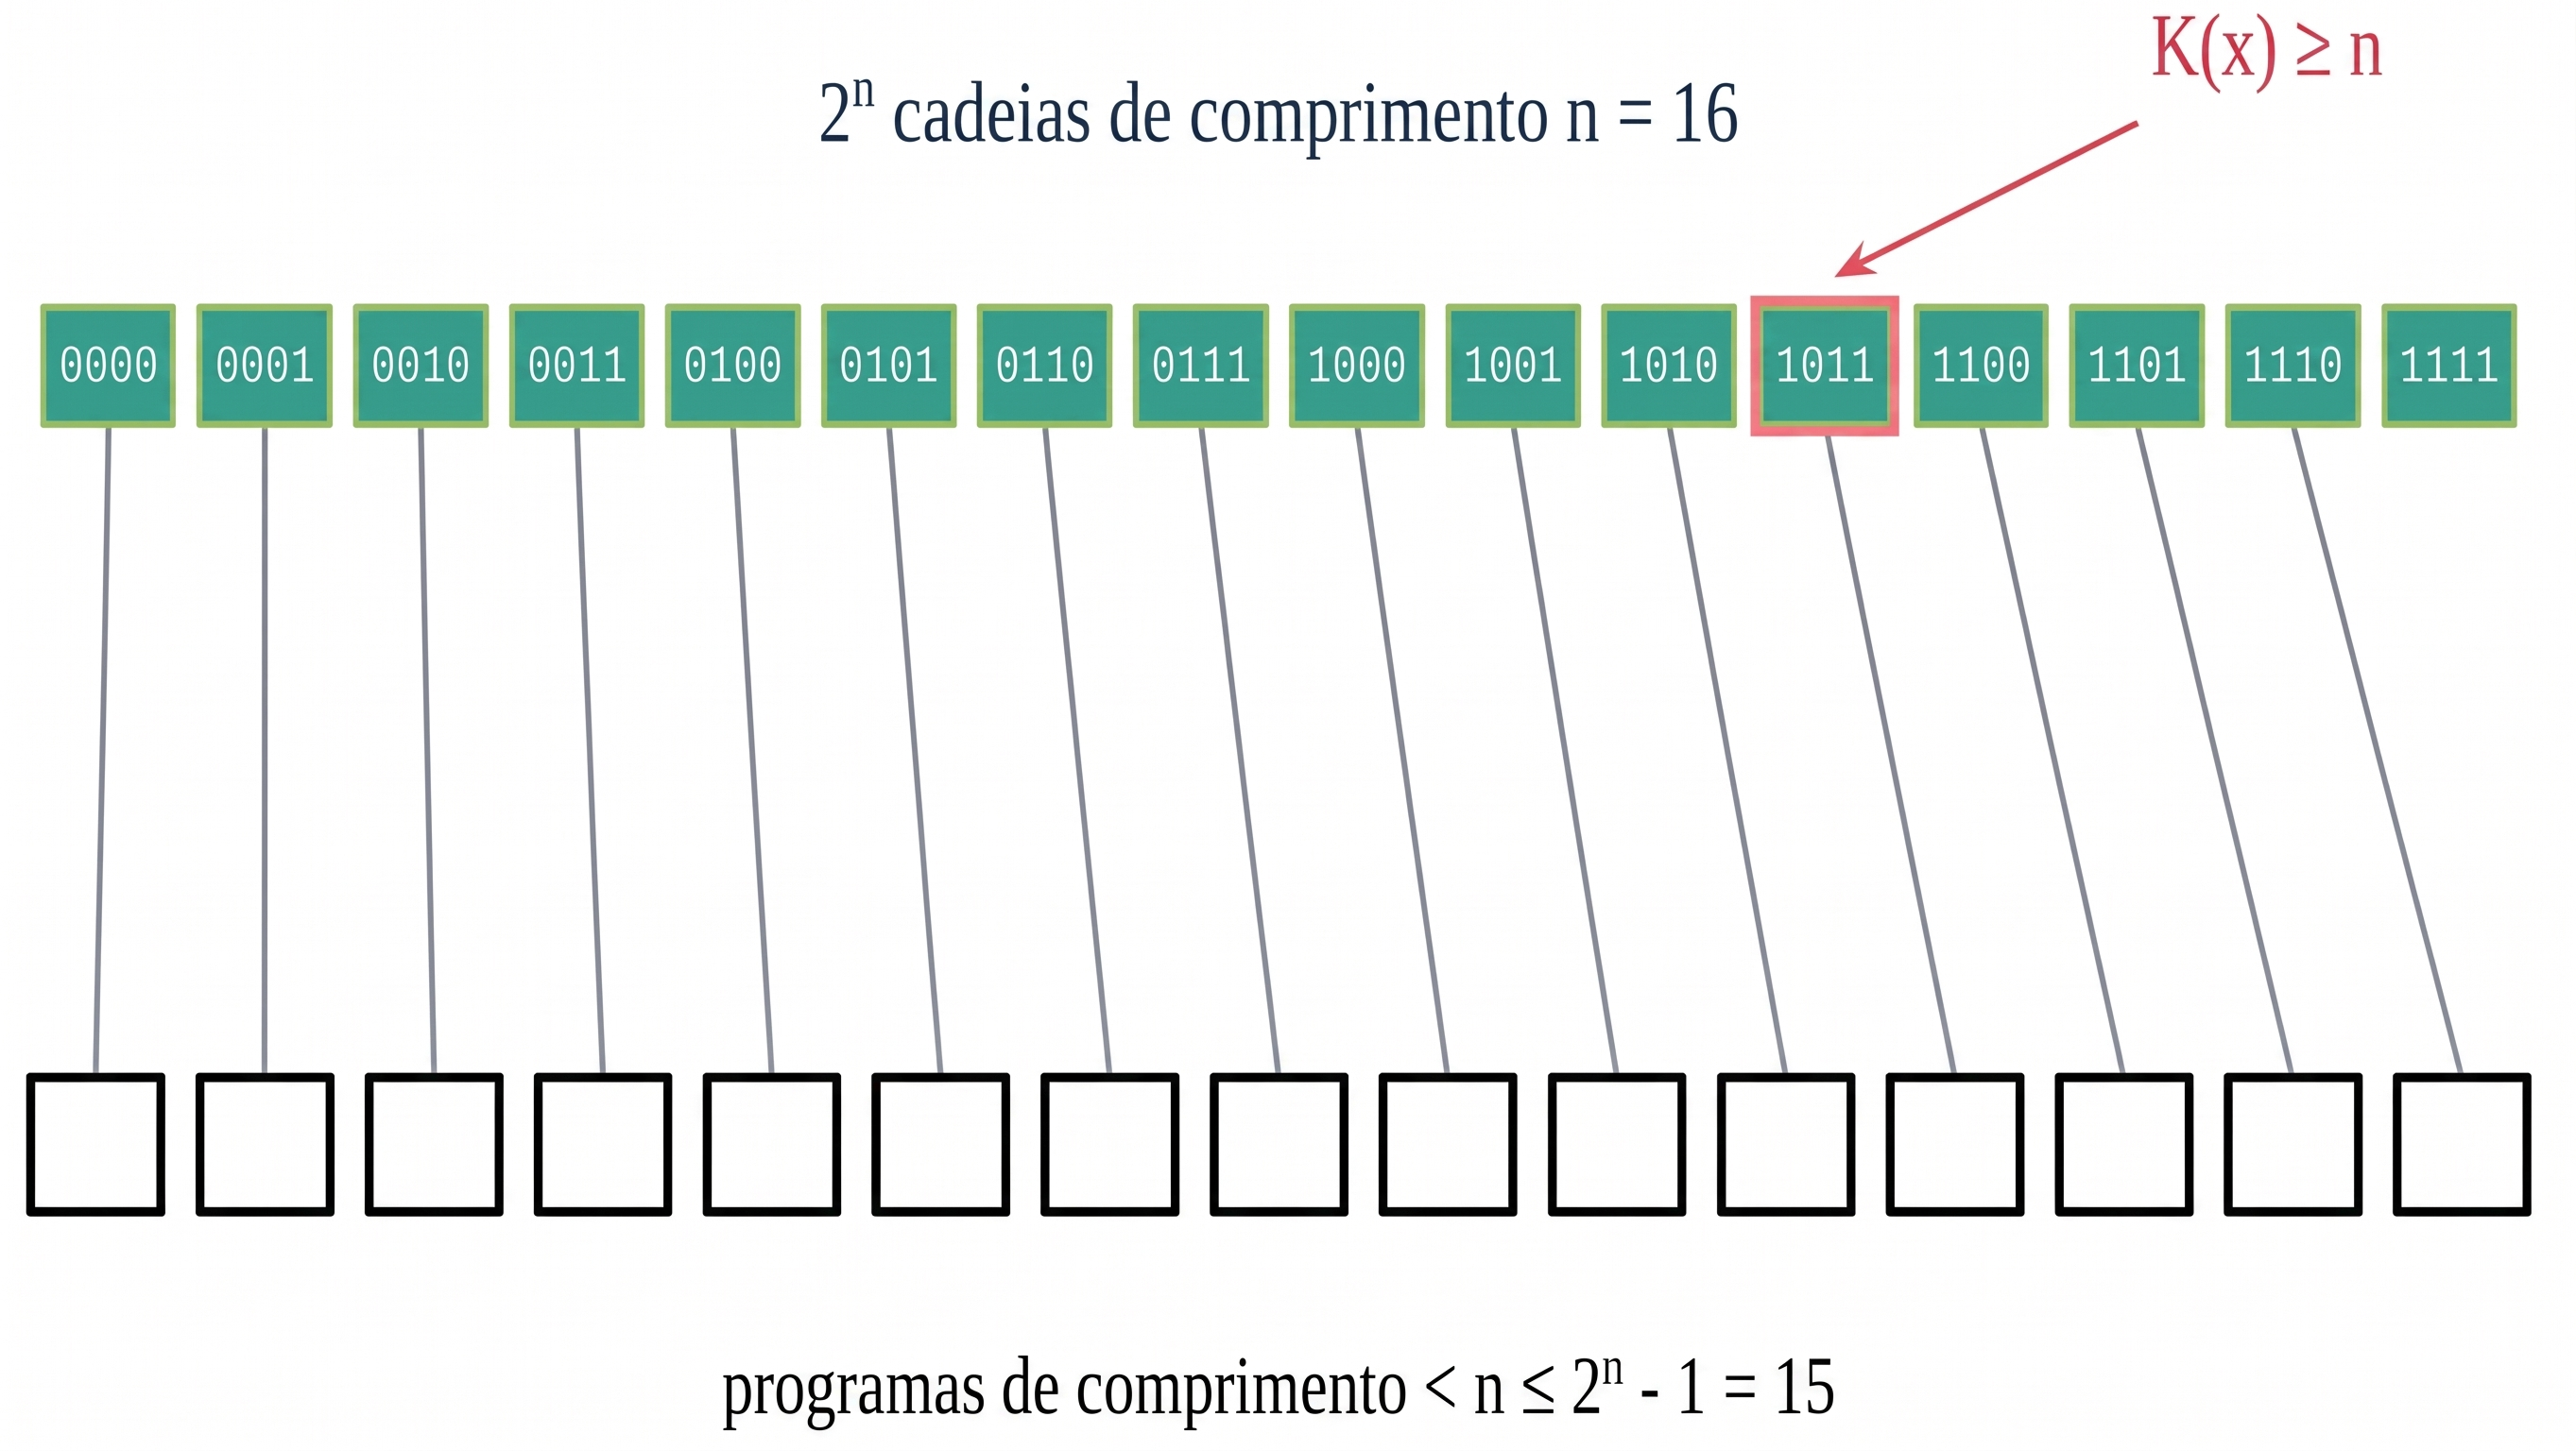
\includegraphics[width=0.93\textwidth]{figures/casa_pombos_example.jpeg}
    \caption{\footnotesize{A violação do Princípio da Casa dos Pombos em relação à Complexidade de Kolmogorov para uma string de $n = 4$.}}
    \label{fig:casa_pombos_example}
\end{figure}
\end{frame}

\section{Problema de Pesquisa}

\begin{frame}{Problema de Pesquisa: O Hiato nas Bibliotecas de Lean 4}
\begin{itemize}
    \item O ecossistema atual do Lean 4 divide-se entre a \textbf{Mathlib} (rica em Teoria dos Números) e a \textbf{Complexitylib} (que formaliza a complexidade descritiva $C_M(x)$ e a existência de strings binárias incompressíveis);
    \item Contudo, a \textbf{Complexitylib} opera puramente sobre strings isoladas (\texttt{List Bool}), carecendo da infraestrutura necessária para demonstrar limites inferiores em estruturas aritméticas:
    \begin{enumerate}
        \item \textbf{Ausência de Códigos Autodelimitados:} Na complexidade simples, concatenar descrições exige esquemas livres de prefixo (\textit{self-terminating codes}) para demarcar fronteiras de decodificação sem perda assintótica;
        \item \textbf{Ponte Informacional-Aritmética:} Acoplar a reconstrução algorítmica à fatoração única e à enumeração de primos da \texttt{Mathlib};
        \item \textbf{Transferência Assintótica:} Formalizar como a redução no comprimento de códigos binários impõe limites inferiores sobre a função de contagem de primos $\pi(n)$.
    \end{enumerate}
\end{itemize}
\end{frame}

\begin{frame}{Problema de Pesquisa}
    \begin{figure}
    \centering
    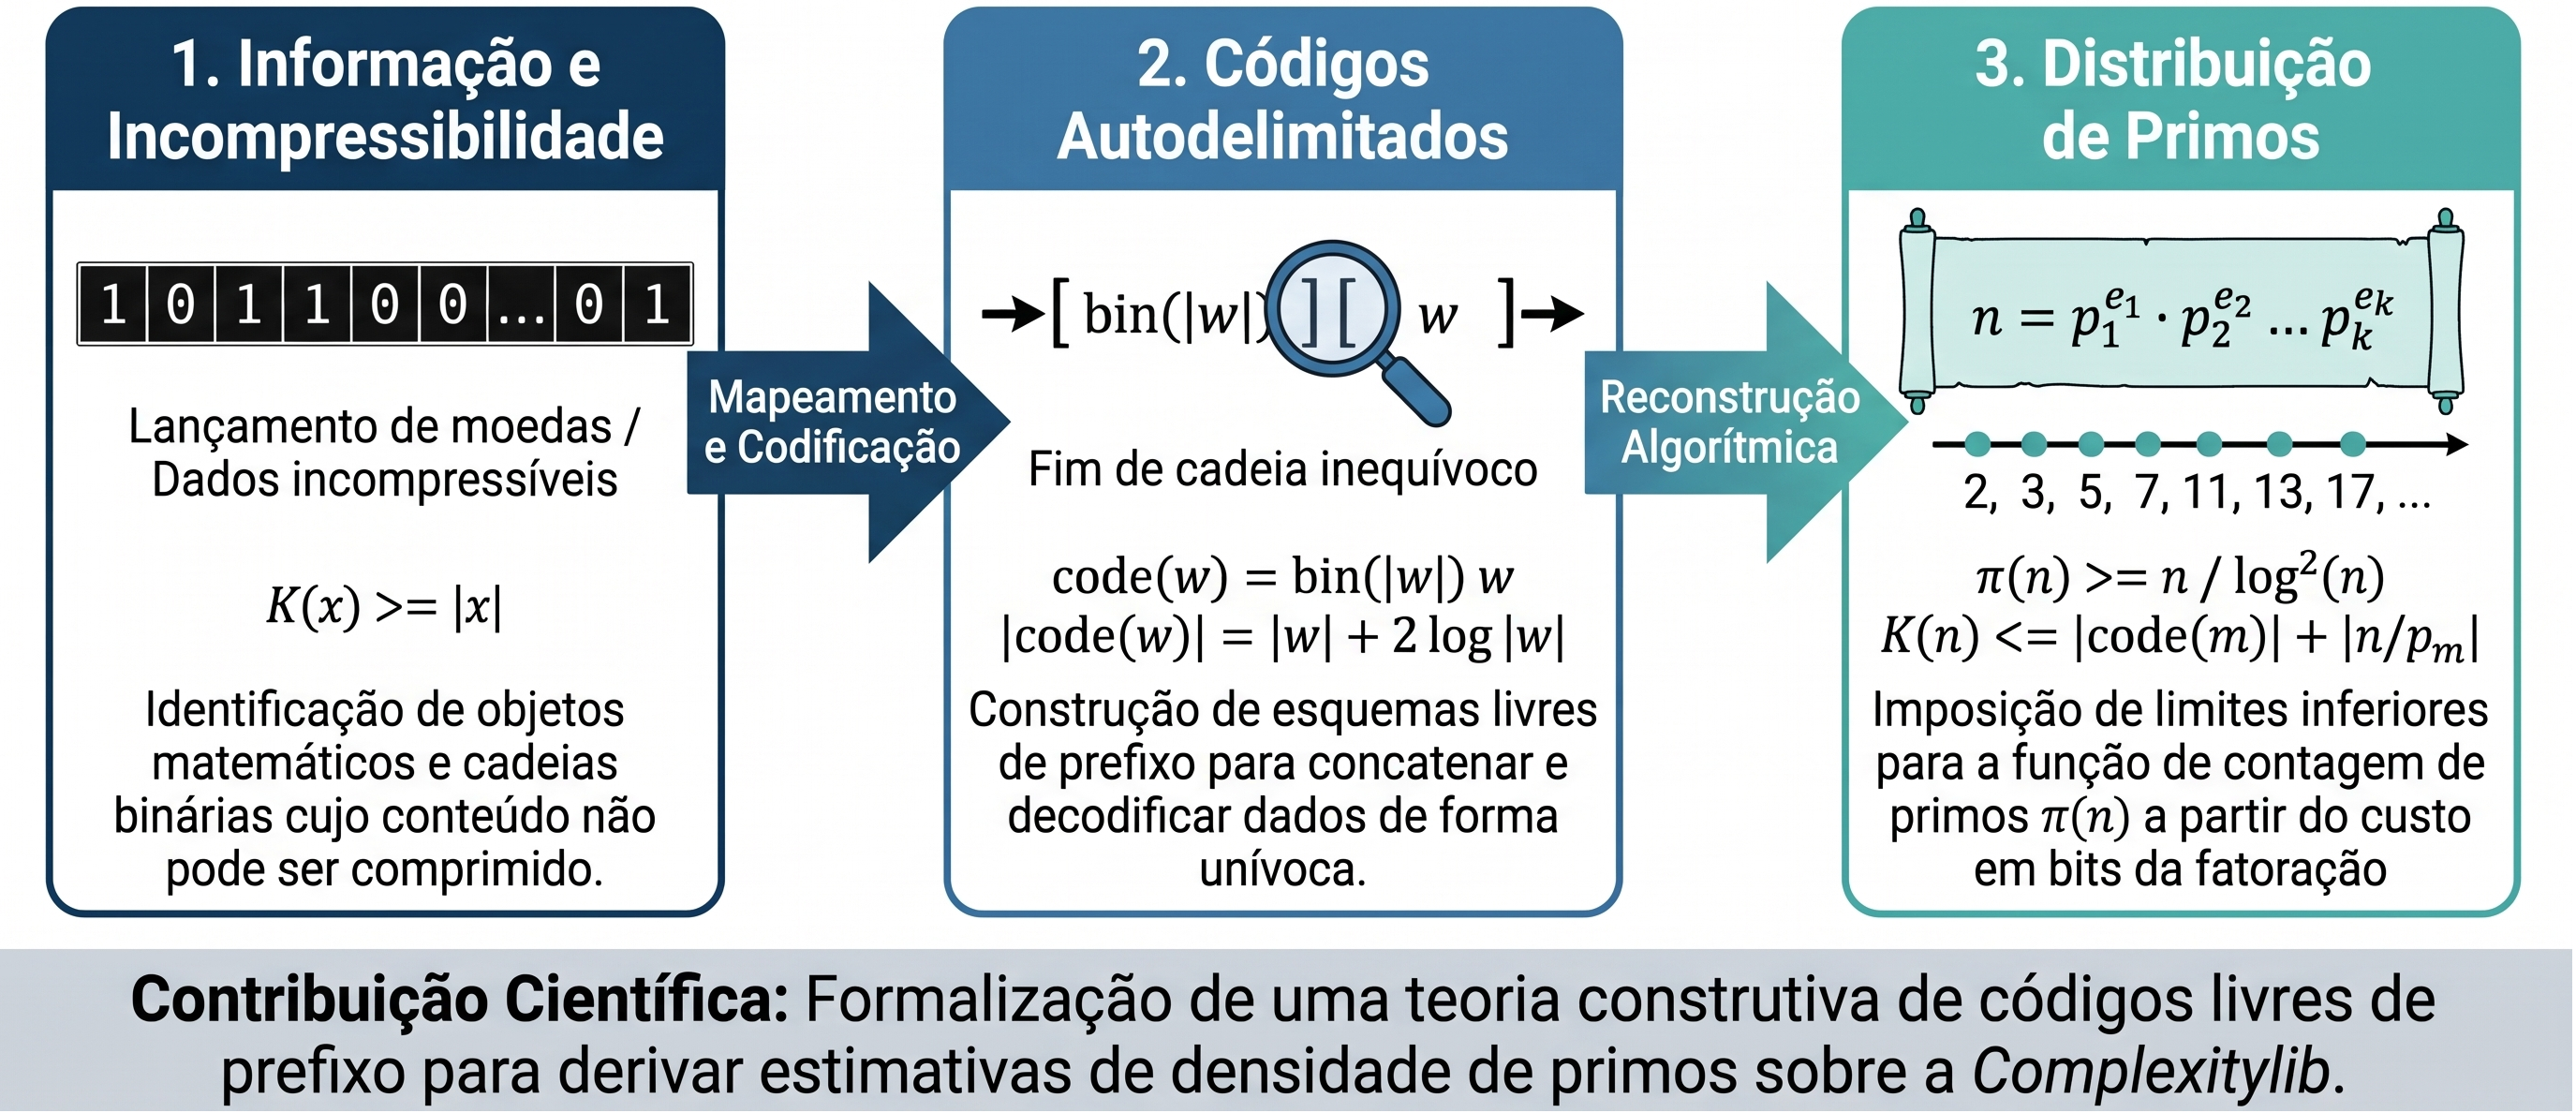
\includegraphics[width=\textwidth]{figures/problem_domain.png}
    \caption{\footnotesize{Arquitetura da formalização: o diagrama ilustra o fluxo metodológico do projeto, detalhando como o princípio abstrato da incompressibilidade de Kolmogorov (1) é estendido por uma teoria de códigos autodelimitados (2) para estabelecer limites inferiores quantitativos na distribuição de números primos (3), evidenciando a extensão proposta sobre a base da \texttt{Complexitylib}.}}
    \label{fig:problem_domain}
    \end{figure}
\end{frame}

\begin{frame}{Problema de Pesquisa}

    \begin{tcolorbox}[pucbox, colframe=red!75!black, title=Problema Central de Pesquisa]
    Como estender a infraestrutura de Complexidade de Kolmogorov da \texttt{\textbf{Complexitylib}} em Lean 4 com esquemas formais de \textbf{codificação autodelimitada} para estabelecer, por pura incompressibilidade algorítmica, a infinitude dos números primos e limites inferiores assintóticos para a sua distribuição $\pi(n)$?
    \end{tcolorbox}
\end{frame}

\section{Objetivos Geral e Específicos}

\begin{frame}{Objetivo Geral}
    \begin{tcolorbox}[pucbox, title=Incompressibilidade Aplicada à Distribuição de Primos]
        {Desenvolver uma formalização mecanicamente verificada em Lean 4 que integre a \textbf{Complexitylib} e a \textbf{Mathlib} por meio de códigos autodelimitados, demonstrando como melhorias na eficiência descritiva de pares de números naturais se traduzem diretamente em limites inferiores progressivamente mais fortes para a função de contagem de primos $\pi(n)$.}
    \end{tcolorbox}
\end{frame}

% --- SLIDE 1 (Itens 1 e 2) ---
\begin{frame}{Objetivos Específicos I}
\begin{enumerate}
    \item \textbf{Ponte Aritmética e Integração com a Complexitylib:}
    \begin{itemize}
        \item Conectar o módulo de incompressibilidade de strings (\texttt{Cslib.Kolmogorov}) à representação binária canônica de números naturais;
        \item Formalizar o princípio de reconstrução injetora como limite superior para a complexidade de Kolmogorov de inteiros;
        \item Demonstrar a infinitude dos números primos via incompressibilidade da codificação da tupla de expoentes de fatoração.
    \end{itemize}
    \medskip
    \item \textbf{Formalização de Códigos Autodelimitados (\textit{Self-Terminating Codes}):}
    \begin{itemize}
        \item Construir funções de codificação livre de prefixo por intercalação de bits ($\overline{w}$) e por prefixação logarítmica de comprimento ($\text{code}(w) = \overline{\text{bin}(|w|)}w$);
        \item Demonstrar formalmente a decodificação única em cadeias concatenadas e caracterizar suas cotas exatas de comprimento;
        \item Generalizar o esquema para codificações autodelimitadas iteradas.
    \end{itemize}
\end{enumerate}
\end{frame}

\begin{frame}{Objetivos Específicos II}
\begin{enumerate}
    \setcounter{enumi}{2}
    \item \textbf{Derivação de Limites Inferiores para $\pi(n)$ (Teorema Fraco dos Primos):}
    \begin{itemize}
        \item Formalizar a reconstrução algorítmica de um inteiro $n$ a partir do índice do seu maior fator primo $m$ e do quociente $n/p_m$;
        \item Estabelecer a redução analítica que converte cotas superiores do $m$-ésimo primo ($p_m$) em limites inferiores para $\pi(n)$;
        \item Demonstrar a cota assintótica $\pi(n) \ge \frac{n}{\log^2 n}$ e sua otimização via códigos iterados.
    \end{itemize}
    \medskip
    \item \textbf{Verificação Mecânica e Contribuição de Biblioteca:}
    \begin{itemize}
        \item Garantir que todas as definições, lemas de comprimento e teoremas de limites inferiores sejam aceitos pelo verificador de tipos do Lean 4 (livres de \texttt{sorry}), estruturando um módulo extensível sobre a \texttt{Complexitylib}.
    \end{itemize}
\end{enumerate}
\end{frame}

\section{Resultados e Entregáveis}

\begin{frame}{Resultados Esperados: Hierarquia de Formalização}
\begin{table}
\centering
\small % Tamanho padrão um pouco menor
\renewcommand{\arraystretch}{1.4} % Boa altura para as frações matematicas

% O resizebox garante que a tabela JAMAIS passará dos limites do slide
\resizebox{\textwidth}{!}{
\begin{tabular}{lp{3.6cm}p{4.4cm}}
\toprule
\textbf{Abordagem} & \textbf{Codificação / Custo} & \textbf{Limite de} $\pi(n)$ \textbf{Verificado} \\ 
\midrule

\textbf{1. Qualitativo} & Expoentes da fatoração \newline $n = p_1^{e_1} \cdots p_k^{e_k}$ & Infinitude de primos \newline ($\pi(n) \to \infty$) \\ \hline

\textbf{2. Elementar} & Intercalação de bits $\overline{w}$ \newline Custo: $2|w|$ & Cota polinomial \newline $\pi(n) \ge \sqrt{n}$ \\ \hline

\textbf{3. Compacto} & Prefixo de tamanho \newline $\text{code}(w) = \overline{\text{bin}(|w|)}w$ \newline Custo: $|w| + 2\log|w|$ & \textbf{Teorema Fraco dos Primos:} \newline $\pi(n) \ge \frac{n}{\log^2 n}$ \\ \hline

\textbf{4. Iterado} & Prefixo recursivo \newline Custo: $\log|w| + 2\log\log|w|$ & Densidade otimizada \newline $\pi(n) \ge \frac{n}{\log n (\log \log n)^2}$ \\ 
\bottomrule
\end{tabular}
}

\vspace{2mm}
\footnotesize
\caption{Impacto da compacidade de códigos no limite de $\pi(n)$.}
\end{table}
\end{frame}
    
\begin{frame}{Entregáveis}
    Dentro do escopo das atividades propostas em \cite{schoning1998kolmogorov}, estão previstos os seguintes entregáveis:
    \medskip

    \begin{tcolorbox}[pucbox, title=Entregáveis do Projeto]
        \begin{itemize}
            \item Definições, lemas e teoremas das soluções dos exercícios, implementados e formalmente verificados em Lean 4 (livres de \texttt{sorry});
            \item Código organizado, documentado e reproduzível a partir de um repositório público no GitHub;
            \item Relatório em PDF com o detalhamento passo a passo das soluções dos exercícios.
        \end{itemize}
    \end{tcolorbox}
\end{frame}

\section{Cronograma}

\begin{frame}{Cronograma de Execução}
\small
\renewcommand{\arraystretch}{1.5}
\begin{table}[]
\centering
\begin{tabular}{@{}p{2.5cm}|p{8.3cm}@{}}
\toprule
\textbf{Período} & \textbf{Meta de Formalização em Lean 4} \\ \midrule

\textbf{02/11 -- 08/11} & \textbf{Integração de Base:} Configuração do ambiente, importação da \texttt{Complexitylib} e adaptação das definições de sequências. \\ \hline

\textbf{09/11 -- 15/11} & \textbf{Códigos Autodelimitados:} Formalização das funções de codificação livres de prefixo ($\overline{w}$ e $\text{code}(w)$) e provas de decodificação única. \\ \hline

\textbf{16/11 -- 22/11} & \textbf{Ponte de Incompressibilidade:} Conexão dos lemas de contagem com a aritmética e formalização da reconstrução bivariada (Ex. 9.2 e 9.3). \\ \hline

\textbf{23/11 -- 29/11} & \textbf{Limites na Distribuição de Primos:} Demonstração da infinitude e do Teorema Fraco dos Primos ($\pi(n) \ge \frac{n}{\log^2 n}$) via incompressibilidade. \\ \hline

\textbf{30/11 -- 04/12} & \textbf{Consolidação e Entrega:} Eliminação de eventuais \texttt{sorry}, elaboração do relatório técnico e submissão do repositório final. \\ 
\bottomrule
\end{tabular}
\end{table}
\end{frame}

% =========================================================================
\section{Referências}
% =========================================================================
\begin{frame}[allowframebreaks]{Referências}
    \bibliography{refs}
\end{frame}
\end{document}

\end{document}